\section{Model}
In this section, we begin to introduce the MiniCPM model that aggregates the aforementioned observations and techniques. 
\label{sec:model}
\begin{table}[htbp]
    \centering
\scalebox{0.90}{
    \begin{tabular}{l|ccccccccc}
    \toprule
        Model & N (B)& $d_m$ & $d_{ff}$ &$d_h$ & $n_q$ & $n_{kv}$& $L$ & Batch size (M)  & Tokens (T)\\
    \midrule
       MiniCPM-1.2B & 1,247,442,432  & 1,536 & 3,840 & 64 & 24 & 8 & 52 & 2M $\rightarrow$ 4M & 1.1T\\
       MiniCPM-2.4B & 2,442,057,984 & 2,304 & 5,760 & 64 & 36 & 36 & 40 & 4M &  1.1T\\
    \bottomrule
    \end{tabular}
}
    \caption{Model configurations for MiniCPM. N (B), $d_m$, $d_{ff}$, $d_h$, $n_q$, $n_{kv}$, $L$, Batch size (M), Tokens (T) represents the number of non-embedding parameters of the model, model hidden dimension, feedforward layer bottleneck dimension, attention head dimension, number of queries, number key/values, number of layers, training batch size, total training tokens.}
    \label{tab:model_configs}
\end{table}
% \vspace{-5mm}

\subsection{Model Details}
\noindent\textbf{Vocabulary.} We use two tokenizers of 122,753 vocabulary size for MiniCPM-2.4B and 73,440 vocabulary for MiniCPM-1.2B. A small vocabulary for 1.2B favors efficiency without harming much performance. Details of the tokenizers are in Appendix~\ref{app:tokenizer}. Including the embedding parameters increases total parameters by 0.3B and 0.2B respectively. 


\noindent\textbf{Shared Input-output Layer.}
For SLM, the embedding takes up a large parameter space. To make the model parameters smaller, we use the Embedding Sharing techniques for both MiniCPM-2.4B and MiniCPM-1.2B.
 % The resulting embedding parameters is $2304 \times 122753 = 0.28B$ for 2.4B and $1536 \times  \sim 0.11B$ for 1.2B. 

\noindent\textbf{Deep-and-thin Network.} We train MiniCPM-2.4B before training MiniCPM-1.2B. When training MiniCPM-2.4B, we adopt a deeper and thinner architecture compared to Phi-2~\citep{Javaheripi2023Phi2} (40 layers compared to 32 layers). Recently, ~\cite{liu2024mobilellm} propose to train deep and thin networks for SLMs, which aligns with our perspective. Therefore, we further make the architecture deeper and thinner for MiniCPM-1.2B. 

\noindent\textbf{Group Query Attention.} We train MiniCPM-2.4B without modification on the attention layer. Whereas we apply Group Query Attention~\citep{ainslie-etal-2023-gqa} to MiniCPM-1.2B, inspired by~\cite{liu2024mobilellm}, to further reduce the parameters number.



\subsection{Training Stages}
The overall training of the MiniCPM base model includes three stages: stable training stage, decay stage, SFT stage~\citep{zhang2023instruction,wei2021finetuned}. Throughout the stages, we use Adam Optimizer~\citep{kingma2014adam}. 

\textbf{Stable Training Stage.}
We utilize around 1T data (see Section~\ref{fig:appdatamixture} for data distribution), with the majority of the data sourced from open datasets. We use the optimal configuration discovered during the model wind tunnel experiments, WSD LRS, with a batch size of 3.93 million and a max learning rate of 0.01.

\textbf{Decay Stage.} We use a mixture of the pretraining data and high-quality SFT data.
For the specific annealing form of the WSD scheduler, we employ exponential annealing, i.e. $f(s-T)=  0.5^{(s-S)/T}$, in which $T$ is set to be 5000 steps (20B tokens).

\textbf{SFT Stage.} We find it still necessary to conduct a separate SFT phase. We utilize SFT data similar to the annealing phase excluding pre-training data and train with approximately 6 billion tokens. The learning rate for SFT is aligned with the one at the end of annealing, and a WSD Scheduler with exponential decay is also employed.


\subsection{Training Data Distribution}
\label{sec:appdatadistrbution}


\begin{figure}[htbp]
    \centering
    \begin{minipage}{0.48\linewidth}
        \centering
        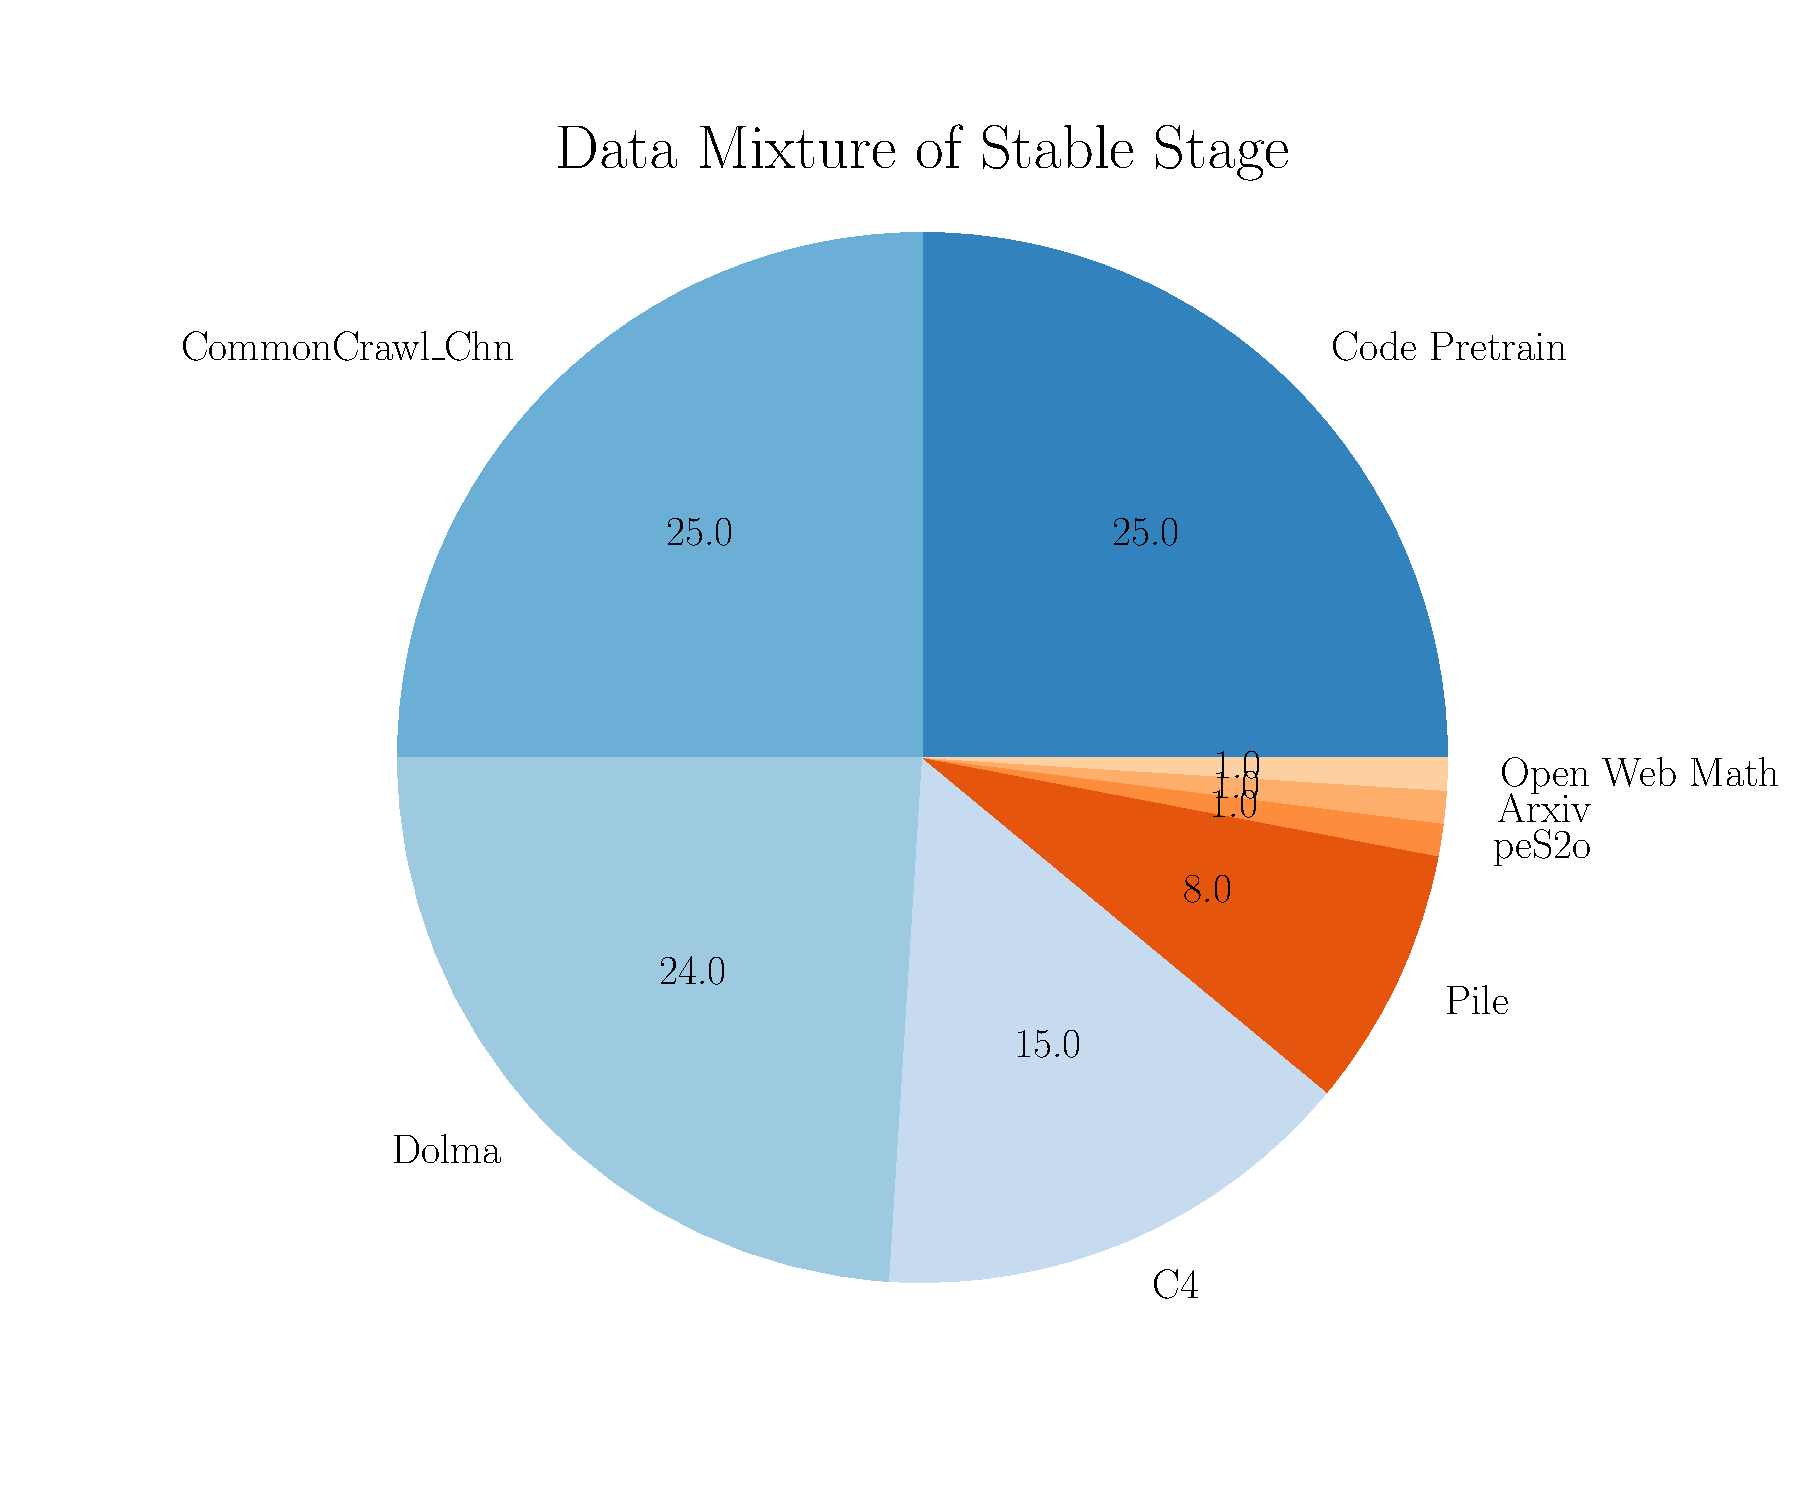
\includegraphics[width=1.0\linewidth]{Fig/stable_mixture.pdf}
    \end{minipage}
    \hfill 
    \begin{minipage}{0.48\linewidth}
        \centering
        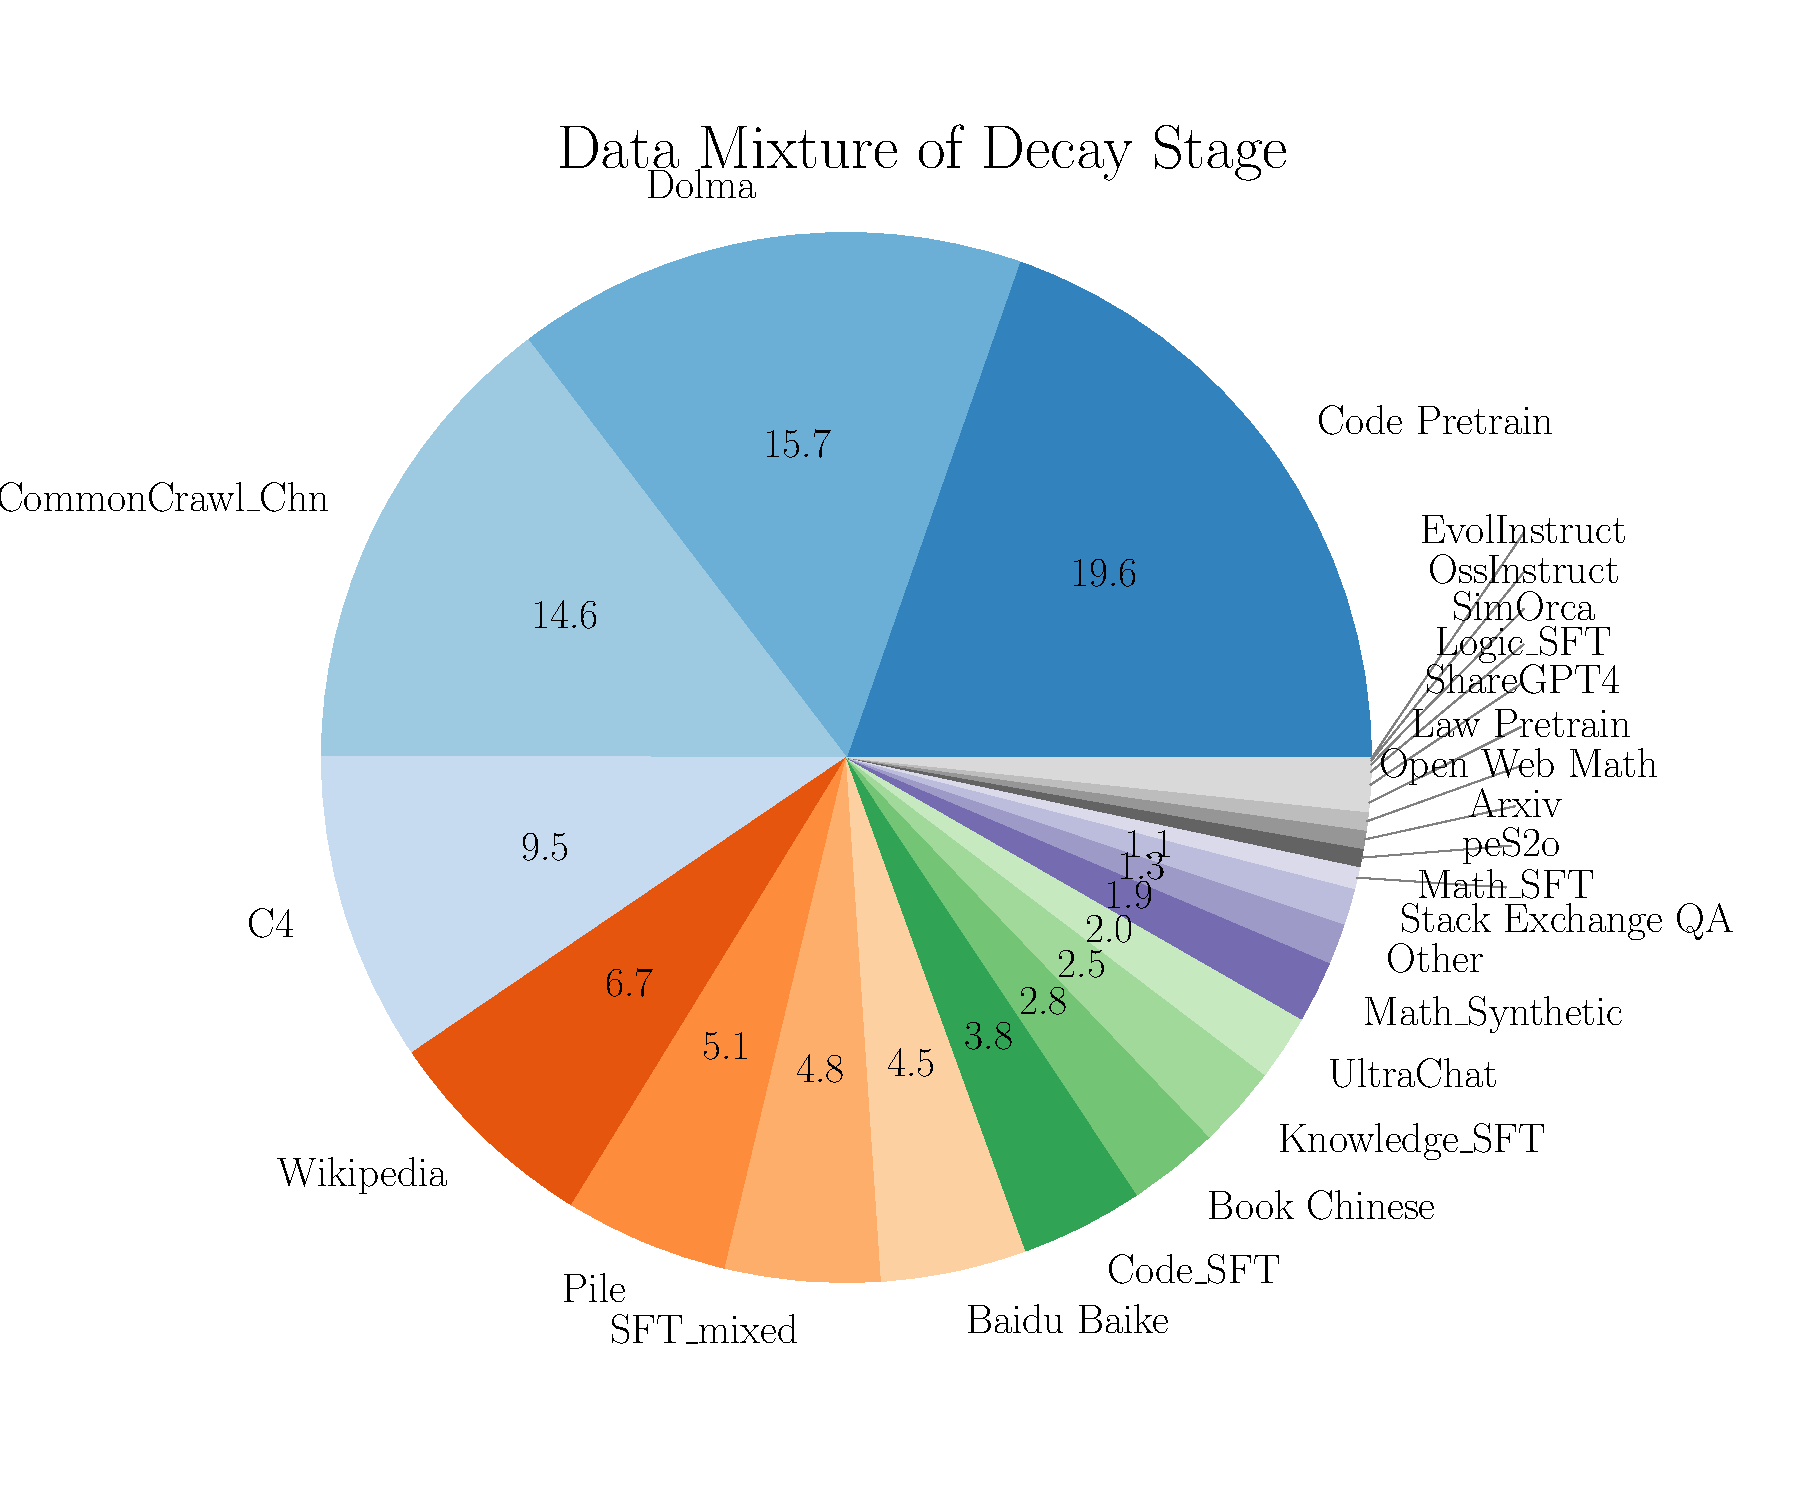
\includegraphics[width=1.0\linewidth]{Fig/decay_data_mixture.pdf}
    \end{minipage}
    \caption{Data mixture of different training stages. The stable stage is shown on the left and the decay stage is shown on the right.}
        \label{fig:appdatamixture}
\end{figure}


We introduce our training data distribution in Figure~\ref{fig:appdatamixture}. In the figure, CommonCrawl\_Chn in a Chinese Corpus is derived from CommonCrawl raw corpus and goes through thorough cleaning. Dolma~\citep{dolma}, C4~\citep{2019t5}, and Pile~\citep{gao2020pile, biderman2022datasheet} are English corpora. They are deduplicated inner corpus and across corpus using MinHash algorithms~\citep{broder1997resemblance}. The Code Pre-train data contains the stack~\citep{Kocetkov2022TheStack} and StarCoder~\cite{li2023starcoder}, with inner deduplication and cross deduplication. In the decay stage, the data mixture contains more diverse data and proprietary data, including UltraChat~\citep{ding2023enhancing}, SlimOrca~\citep{SlimOrca, SlimOrcaDedup}, OssInstruct~\citep{wei2023magicoder}, EvolInstruct~\citep{xu2023wizardlm}. The data with the suffix SFT is our proprietary data including LeetCode questions, Kindergarten through 12th grade (K12) textbooks and questions, etc. 


\subsection{Training Loss}

\definecolor{darkgreen}{HTML}{476E6B}

The overall training loss on the C4 dataset is shown in Figure~\ref{fig:loss_c4}. We can see that as expected in the preliminary experiments, the loss decreases sharply in the decay stage. Since we use the exponential decay, the loss still drops after the learning rate drops below 10\% of the max learning rate. However, since we continue to SFT the model after the decay stage, we do not utilize the final checkpoints. The checkpoints we finetune from are shown in the last checkpoint of \textcolor{darkgreen}{dark green} segment. The first drop in MiniCPM-1.2B is the result of enlarging batch size, which might have a similar effect as decreasing learning rate~\citep{smith2017don}.


\definecolor{orange}{HTML}{FFA500}



\begin{figure}[htbp]
    \centering
    % First minipage for the first figure
    \begin{minipage}{0.48\linewidth}
        \centering
        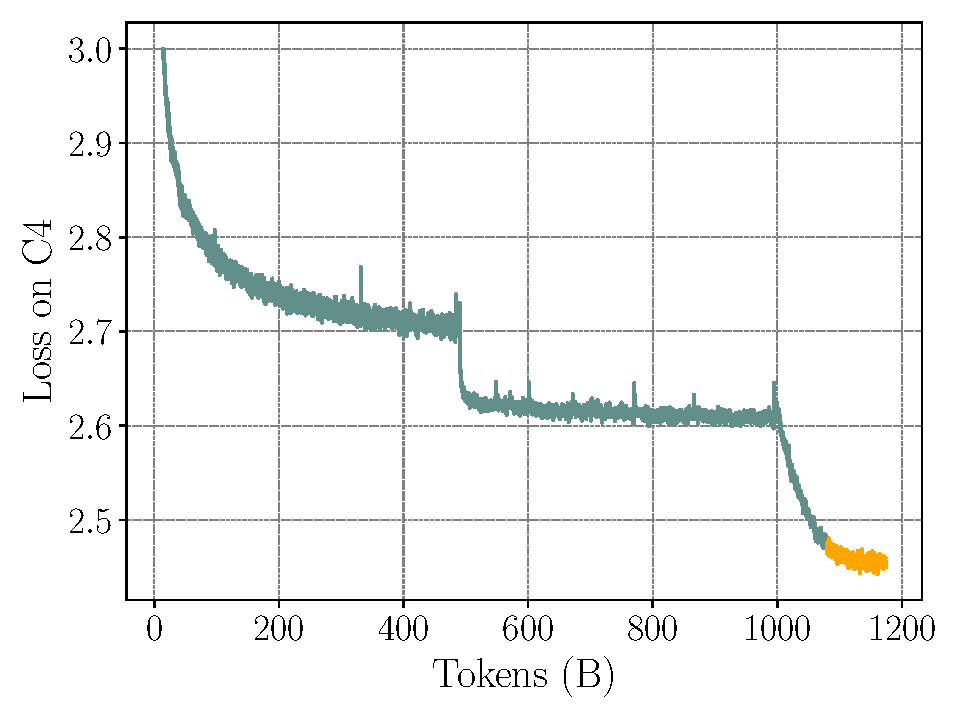
\includegraphics[width=0.9\linewidth]{Fig/1.2B_c4_loss_smoothed.pdf}
    \end{minipage}
    \hfill % This adds a little space between the two figures
    % Second minipage for the second figure
    \begin{minipage}{0.48\linewidth}
        \centering
        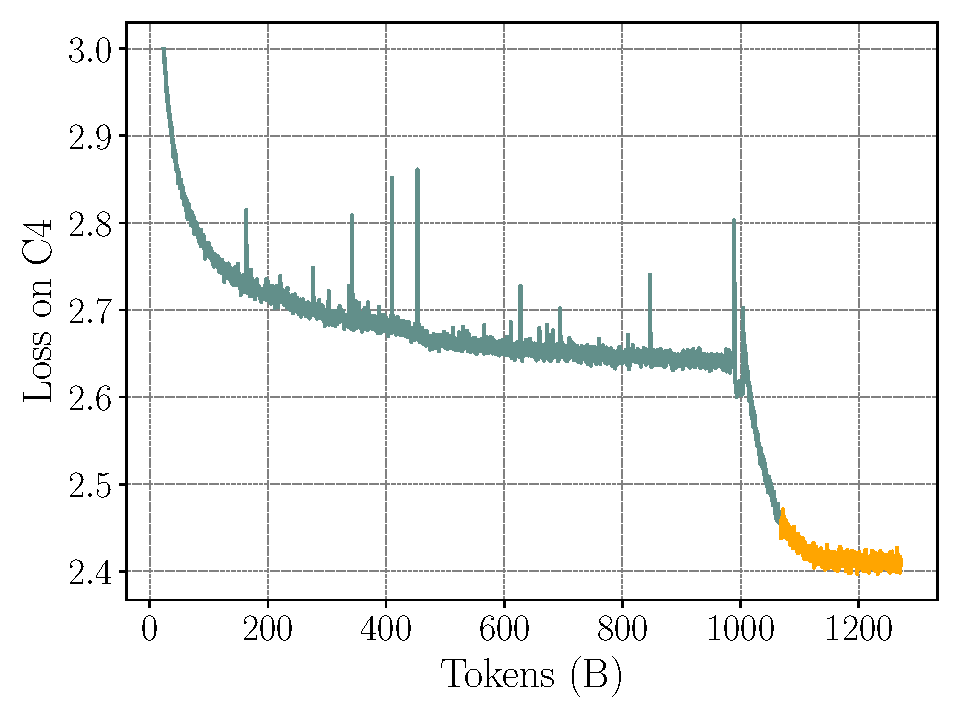
\includegraphics[width=0.9\linewidth]{Fig/2.4B_c4_loss_smoothed.pdf}
    \end{minipage}
     \caption{Loss curve on C4 dataset for MiniCPM-1.2B (Left) and MiniCPM-2.4B (Right). The  \textcolor{orange}{orange} segment at the tail of the loss curve represents the remaining decay process, which is not utilized in the released version of MiniCPM.}
        \label{fig:loss_c4}
\end{figure}

\begin{table}[!htbp]
    \centering
\scalebox{0.90}{
    \begin{tabular}{lm{1.2cm}m{1.2cm}m{1.2cm}m{1.7cm}m{1.2cm}m{1.2cm}m{1.2cm}m{1.2cm}}
\toprule
\textbf{Model} & \textbf{C-Eval} & \textbf{CMMLU} & \textbf{MMLU} & \textbf{HumanEval} & \textbf{MBPP} & \textbf{GSM8K} & \textbf{MATH}\\
\midrule
Llama2-7B & 32.42 & 31.11 & 44.32 & 12.20 & 27.17 & 13.57 & 1.80\\
Qwen-7B & 58.96 & 60.35 & 57.65 & 17.07 & 42.15 & 41.24 & 5.34\\
Deepseek-7B  & 42.82 & 44.45 & 47.82 & 20.12 & 41.45 & 15.85 & 1.53 \\
Mistral-7B  & 46.12 & 42.96 & 62.69 & 27.44 & 45.20 & 33.13 & 5.00 \\
Gemma-7B  & 42.57 & 44.20 & 60.83 & 38.41 & 50.12 & 47.31 & 6.18\\
\midrule
Llama2-13B  & 37.32 & 37.06 & 54.71 & 17.07 & 32.55 & 21.15 & 2.25\\
MPT-30B  & 29.34 & 32.09 & 46.56 & 21.95 & 35.36 & 10.31 & 1.56 \\
Falcon-40B & 40.29 & 41.57 & 53.53 & 24.39 & 36.53 & 22.44 & 1.92 \\
\midrule
TinyLlama-1.1B & 25.02 & 24.03 & 24.3 & 6.71 & 19.91 & 2.27 & 0.74 \\
Qwen-1.8B & 49.81 & 45.32 & 43.37 & 7.93 & 17.8 & 19.26& 2.42 \\
Qwen1.5-1.8B & \textbf{55.00} & 50.85 & 43.81 & 5.49 & 24.82 & 26.16 & 3.25 \\
Gemini Nano-3B & - & - & - & - & 27.20 & 22.80 & - \\
StableLM-Zephyr-3B & 30.34 & 30.89 & 45.90 & 35.37 & 31.85 & 52.54 & 12.12\\
Phi-2(2B) & 23.37 & 24.18 & 52.66 & 47.56 & \textbf{55.04} & \textbf{57.16} & 3.50 \\
Gemma-2B & 29.26 & 28.56 & 38.49 & 24.39 & 29.74 & 16.83 & 3.34\\
\midrule
\textbf{MiniCPM-1.2B} & 49.14 & 46.81 & 49.63  & 44.51  & 32.75 & 31.77 &  10.60 \\
\textbf{MiniCPM-2.4B} & 51.13 & \textbf{51.07} & \textbf{53.46} & \textbf{50.00 }& 47.31 & 53.83 & \textbf{10.24}\\
\bottomrule
\end{tabular}
}
\scalebox{0.90}{
 \begin{tabular}{lm{1.2cm}m{1.2cm}m{1.2cm}m{1.7cm}m{1.2cm}m{1.2cm}m{1.2cm}m{1.2cm}}
\textbf{Model}  & \textbf{BBH} &\textbf{ARC-e} & \textbf{ARC-c} & \textbf{HellaSwag} & \textbf{Avg} & \textbf{Avg$_{\text{en}}$} & \textbf{Avg$_{\text{chn}}$} \\
\midrule
Llama2-7B  & 33.23 & 75.25$^{\dag}$ & 42.75 & 75.62$^{\dag}$ & 35.40 & 36.21 & 31.77 \\
Qwen-7B  & 37.75 & 83.42 & 64.76 & 75.32$^{\dag}$ & 49.46 & 47.19 & 59.66 \\
Deepseek-7B  & 33.38 & 74.58$^{\dag}$ & 42.15$^{\dag}$ & 75.45$^{\dag}$ & 39.96 & 39.15 & 43.64 \\
Mistral-7B & 41.06 & 83.92 & 70.73 & 80.43$^{\dag}$ & 48.97 & 49.96 & 44.54 \\
Gemma-7B  & 39.19 & 89.35 & 76.79 & 79.47 & 52.22 & 54.18 & 43.39 \\
\midrule
Llama2-13B & 37.92 & 78.87$^{\dag}$ & 58.19 & 79.23$^{\dag}$ & 41.48 & 42.44 & 37.19 \\
MPT-30B  & 38.22 & 78.66$^{\dag}$ & 46.08$^{\dag}$ & 79.72$^{\dag}$ & 38.17 & 39.82 & 30.72 \\
Falcon-40B & 36.24 & 81.94$^{\dag}$ & 57.68 & 83.26$^{\dag}$ & 43.62 & 44.21 & 40.93 \\
\midrule
TinyLlama-1.1B  & 28.78 & 60.77$^{\dag}$ & 28.15$^{\dag}$ & 58.33$^{\dag}$ & 25.36 & 25.55 & 24.53 \\
Qwen-1.8B  & 29.07 & 63.97$^{\dag}$ & 43.69 & 59.28$^{\dag}$ & 34.72 & 31.87 & 47.57 \\
Qwen1.5-1.8B  & 28.82 & 64.86 & 45.56 & 59.39 & 37.09 & 33.57 & \textbf{52.93} \\
Gemini Nano-3B & 42.40 & - & - & - & - & - & - \\
StableLM-Zephyr-3B  & 37.68 & 73.78 & 55.38 & 71.87$^{\dag}$ & 43.46 & 46.32 & 30.62 \\
Phi-2(2B)  & \textbf{43.39} & \textbf{86.11} & \textbf{71.25} & \textbf{73.07$^{\dag}$} & 48.84 & \textbf{54.42} & 23.78 \\
Gemma-2B  & 30.93 & 74.33 & 40.70 & 69.51 & 35.10 & 36.47 & 28.91\\
\midrule
\textbf{MiniCPM-1.2B}  & 34.70 & 80.93 & 66.81 &  \textbf{54.72} &  45.67 & 45.16 & 47.98 \\
\textbf{MiniCPM-2.4B}  & 36.87 & 85.44 & 68.00 & 68.25 & \textbf{52.33} & 52.60 & 51.10 \\
\bottomrule
\end{tabular}
}
\caption{Benchmark Score of MiniCPM-2.4B and MiniCPM-1.2B (both without RLHF). The two tables are continuous horizontally. \textbf{Avg} is over all dataset in the table, \textbf{Avg$_{\text{chn}}$} is the average of C-Eval and CMMLU while \textbf{Avg$_{\text{en}}$} is the average of remaining datasets. $\dag$ means the result is tested using PPL metrics. \textbf{Bold} numbers represent the best score among the SLMs. Results of Gemini Nano-3B are borrowed from ~\cite{team2023gemini}.}
\label{tab:benchmark_without_rlhf}
\end{table}
\vspace{-5mm}


\subsection{Evaluation}
\label{sec:evaluation}
The overall evaluation utilizes our open-source tool UltraEval\footnote{https://ultraeval.openbmb.cn/home}. UltraEval is an open-source framework for assessing the capabilities of foundation models. It provides a lightweight and user-friendly evaluation system, supporting performance assessment for mainstream large models, and catering to the rapid evaluation needs of model training teams. The underlying inference and acceleration use the open-source framework vLLM~\citep{kwon2023efficient}, and the dataset includes commonly used datasets: MMLU~\citep{hendrycks2020measuring} for English knowledge, CMMLU~\citep{li2024cmmlu} and C-Eval~\citep{huang2024c} for Chinese knowledge, HumanEval~\citep{chen2021evaluating} and MBPP~\citep{austin2021program} for coding, GSM8K~\citep{cobbe2021training} and MATH~\citep{hendrycks2021measuring} for mathematics, and HellaSwag~\citep{zellers2019hellaswag}, ARC-e~\citep{clark2018think}, ARC-c~\citep{clark2018think} for commonsense reasoning, and BBH~\citep{suzgun2022challenging} for logic reasoning. 

Due to the difficulty of standardizing evaluations for large models and the lack of publicly available prompts and test codes for many models' evaluations, we try our best to adapt the evaluation methods to suit various model types. Specifically, we start from a standardized input prompt during testing and adjust it according to each model's appropriate input-output template. The \textbf{evaluation scripts and prompts are also open-source} in our repository, and we welcome developers to continually improve our evaluation methods.

When testing QA tasks (ARC-e, ARC-c, HellaSwag), two approaches are typically employed. The first involves using Perplexity (PPL): we extend each option as the continuation of the question and use the PPL of the option as the selection criterion. The second is direct generation, where the model directly outputs answer options. We observe significant differences in results obtained using these two methods.  MiniCPM performs similarly in direct generation and PPL tests, with better performance in direct generation. On the other hand, Mistral-7B-v0.1 performs better in PPL tests but exhibits poorer performance in direct generation. To address this phenomenon, when reporting the scores for each model, we adopt the score from the evaluation method that yields the highest score, ensuring fairness in comparison.

The overall evaluation results are in Table~\ref{tab:benchmark}. Overall, on the mentioned datasets, we have several observations. (1) On average, MiniCPM-2.4B ranks the highest among all the SLMs. (2) MiniCPM-2.4B performs similarly to Mistral-7B-v0.1 in English but significantly outperforms Mistral-7B-v0.1 in Chinese. (3) MiniCPM-2.4B outperforms Llama2-13B except in MMLU, BBH, and HellaSwag, while MiniCPM-1.2B outperforms Llama2-7B except in HellaSwag. (4)Generally, BBH is harder for SLMs than LLMs compared to another knowledge-oriented dataset, demonstrating that reasoning ability might be more dependent on model size than knowledge. (5) Among SLMs, Phi-2 performance is on par with MiniCPM on academic-oriented datasets. This might be because their training data mostly involves textbook-style data that emphasize educational and academic scenarios. Since our pre-training data covers more distribution, we think MiniCPM is better at knowledge and ability coverage, which can be seen in Appendix~\ref{app:cases}.




\section{MiniCPM Family}
In this section, we introduce the other models that build on MiniCPM base models. Specifically, we trained the aligned model, long-context model, and MoE model for MiniCPM 2.4B.

\subsection{MiniCPM-DPO}
\label{app:rlhf}
After SFT, we employ \uline{DPO}~\citep{rafailov2024direct} for human preference alignment of the model. During this stage, \uline{UltraFeedback}~\citep{cui2023ultrafeedback} is utilized as the primary alignment dataset, and a proprietary preference dataset is constructed to enhance the model's code and mathematical capabilities. We conduct one epoch of DPO training with \uline{a learning rate of $1\times 10^{-5}$} and utilize a Cosine LRS since we have a pre-defined training step.

\begin{table}[htbp]
    \centering
\scalebox{0.87}{

\begin{tabular}{lccccccccc}
\toprule
\textbf{Model} & \textbf{C-Eval} & \textbf{CMMLU} & \textbf{MMLU} & \textbf{HumanEval} & \textbf{MBPP} & \textbf{GSM8K} & \textbf{MATH}\\
\midrule
ChatGLM2-6B & 52.05 & 49.21 & 45.77 & 10.37 & 9.38 & 22.74 & 5.96 \\
Mistral-7B-Instruct-v0.1 & 38.06 & 36.96 & 53.56 & 29.27 & 39.34 & 28.73 & 3.48\\
Mistral-7B-Instruct-v0.2 & 42.55 & 41.92 & 60.51 & 36.59 & 48.95 & 40.49 & 4.95 \\
Qwen-7B-Chat & 58.57 & 57.23 & 56.03 & 15.85 & 40.52 & 42.23 & 8.3\\
Yi-6B-Chat & 70.88 & 71.11 & 62.95 & 14.02 & 28.34 & 36.54 & 3.88\\
Baichuan2-7B-Chat & 53.28 & 53.50 & 53.00 & 21.34 & 32.32 & 25.25 & 6.32\\
Deepseek-7B-chat & 46.95 & 49.72 & 51.67 & 40.85 & 48.48 & 48.52 & 4.26 \\
Llama2-7B-Chat & 34.54 & 32.64 & 47.64 & 14.02 & 27.40 & 21.15 & 2.08 \\
\midrule
\textbf{MiniCPM-2.4B-DPO}  & 48.64 & 48.37 & 53.05 & 51.22 & 48.01 & 53.37 & 9.86\\
\bottomrule
\end{tabular}
}

\scalebox{0.88}{
\begin{tabular}{lccccccc}
\toprule
\textbf{Model}  & \textbf{BBH} &\textbf{ ARC-e} & \textbf{ARC-c} & \textbf{HellaSwag} & \textbf{Avg} & \textbf{Avg$_{\text{en}}$} & \textbf{Avg$_{\text{chn}}$}  \\
\midrule
ChatGLM2-6B  & 32.60 & 74.45 & 56.82 & 58.48$^{\dag}$ & 37.98 & 35.17 & 50.63 \\
Mistral-7B-Instruct-v0.1  & 39.52 & 81.61 & 63.99 & 73.47$^{\dag}$ & 44.36 & 45.89 & 37.51 \\
Mistral-7B-Instruct-v0.2  & 39.81 & 86.28 & 73.38 & 84.55$^{\dag}$ & 50.91 & 52.83 & 42.24 \\
Qwen-7B-Chat  & 37.34 & 64.44$^{\dag}$ & 39.25$^{\dag}$ & 74.52$^{\dag}$ & 44.93 & 42.05 & 57.90 \\
Yi-6B-Chat  & 37.43 & 84.89 & 70.39 & 74.60$^{\dag}$ & 50.46 & 45.89 & 71.00 \\
Baichuan2-7B-Chat  & 37.46 & 79.63 & 60.15 & 69.23$^{\dag}$ & 44.68 & 42.74 & 53.39 \\
Deepseek-7B-chat  & 35.70 & 76.85 & 63.05 & 76.68$^{\dag}$ & 49.34 & 49.56 & 48.34 \\
Llama2-7B-Chat  & 35.54 & 74.28 & 54.78 & 75.65$^{\dag}$ & 38.16 & 39.17 & 33.59 \\
\midrule
\textbf{MiniCPM-2.4B-DPO}  & 36.22 & 85.02 & 68.17 & 65.67 & 51.60 & 52.29 & 48.51 \\
\bottomrule
\end{tabular}
}
\caption{Benchmark scores for MiniCPM-2.4B-DPO compared with larger chat models.}
\label{tab:benchmark}
\end{table}

\begin{figure}
    \centering
    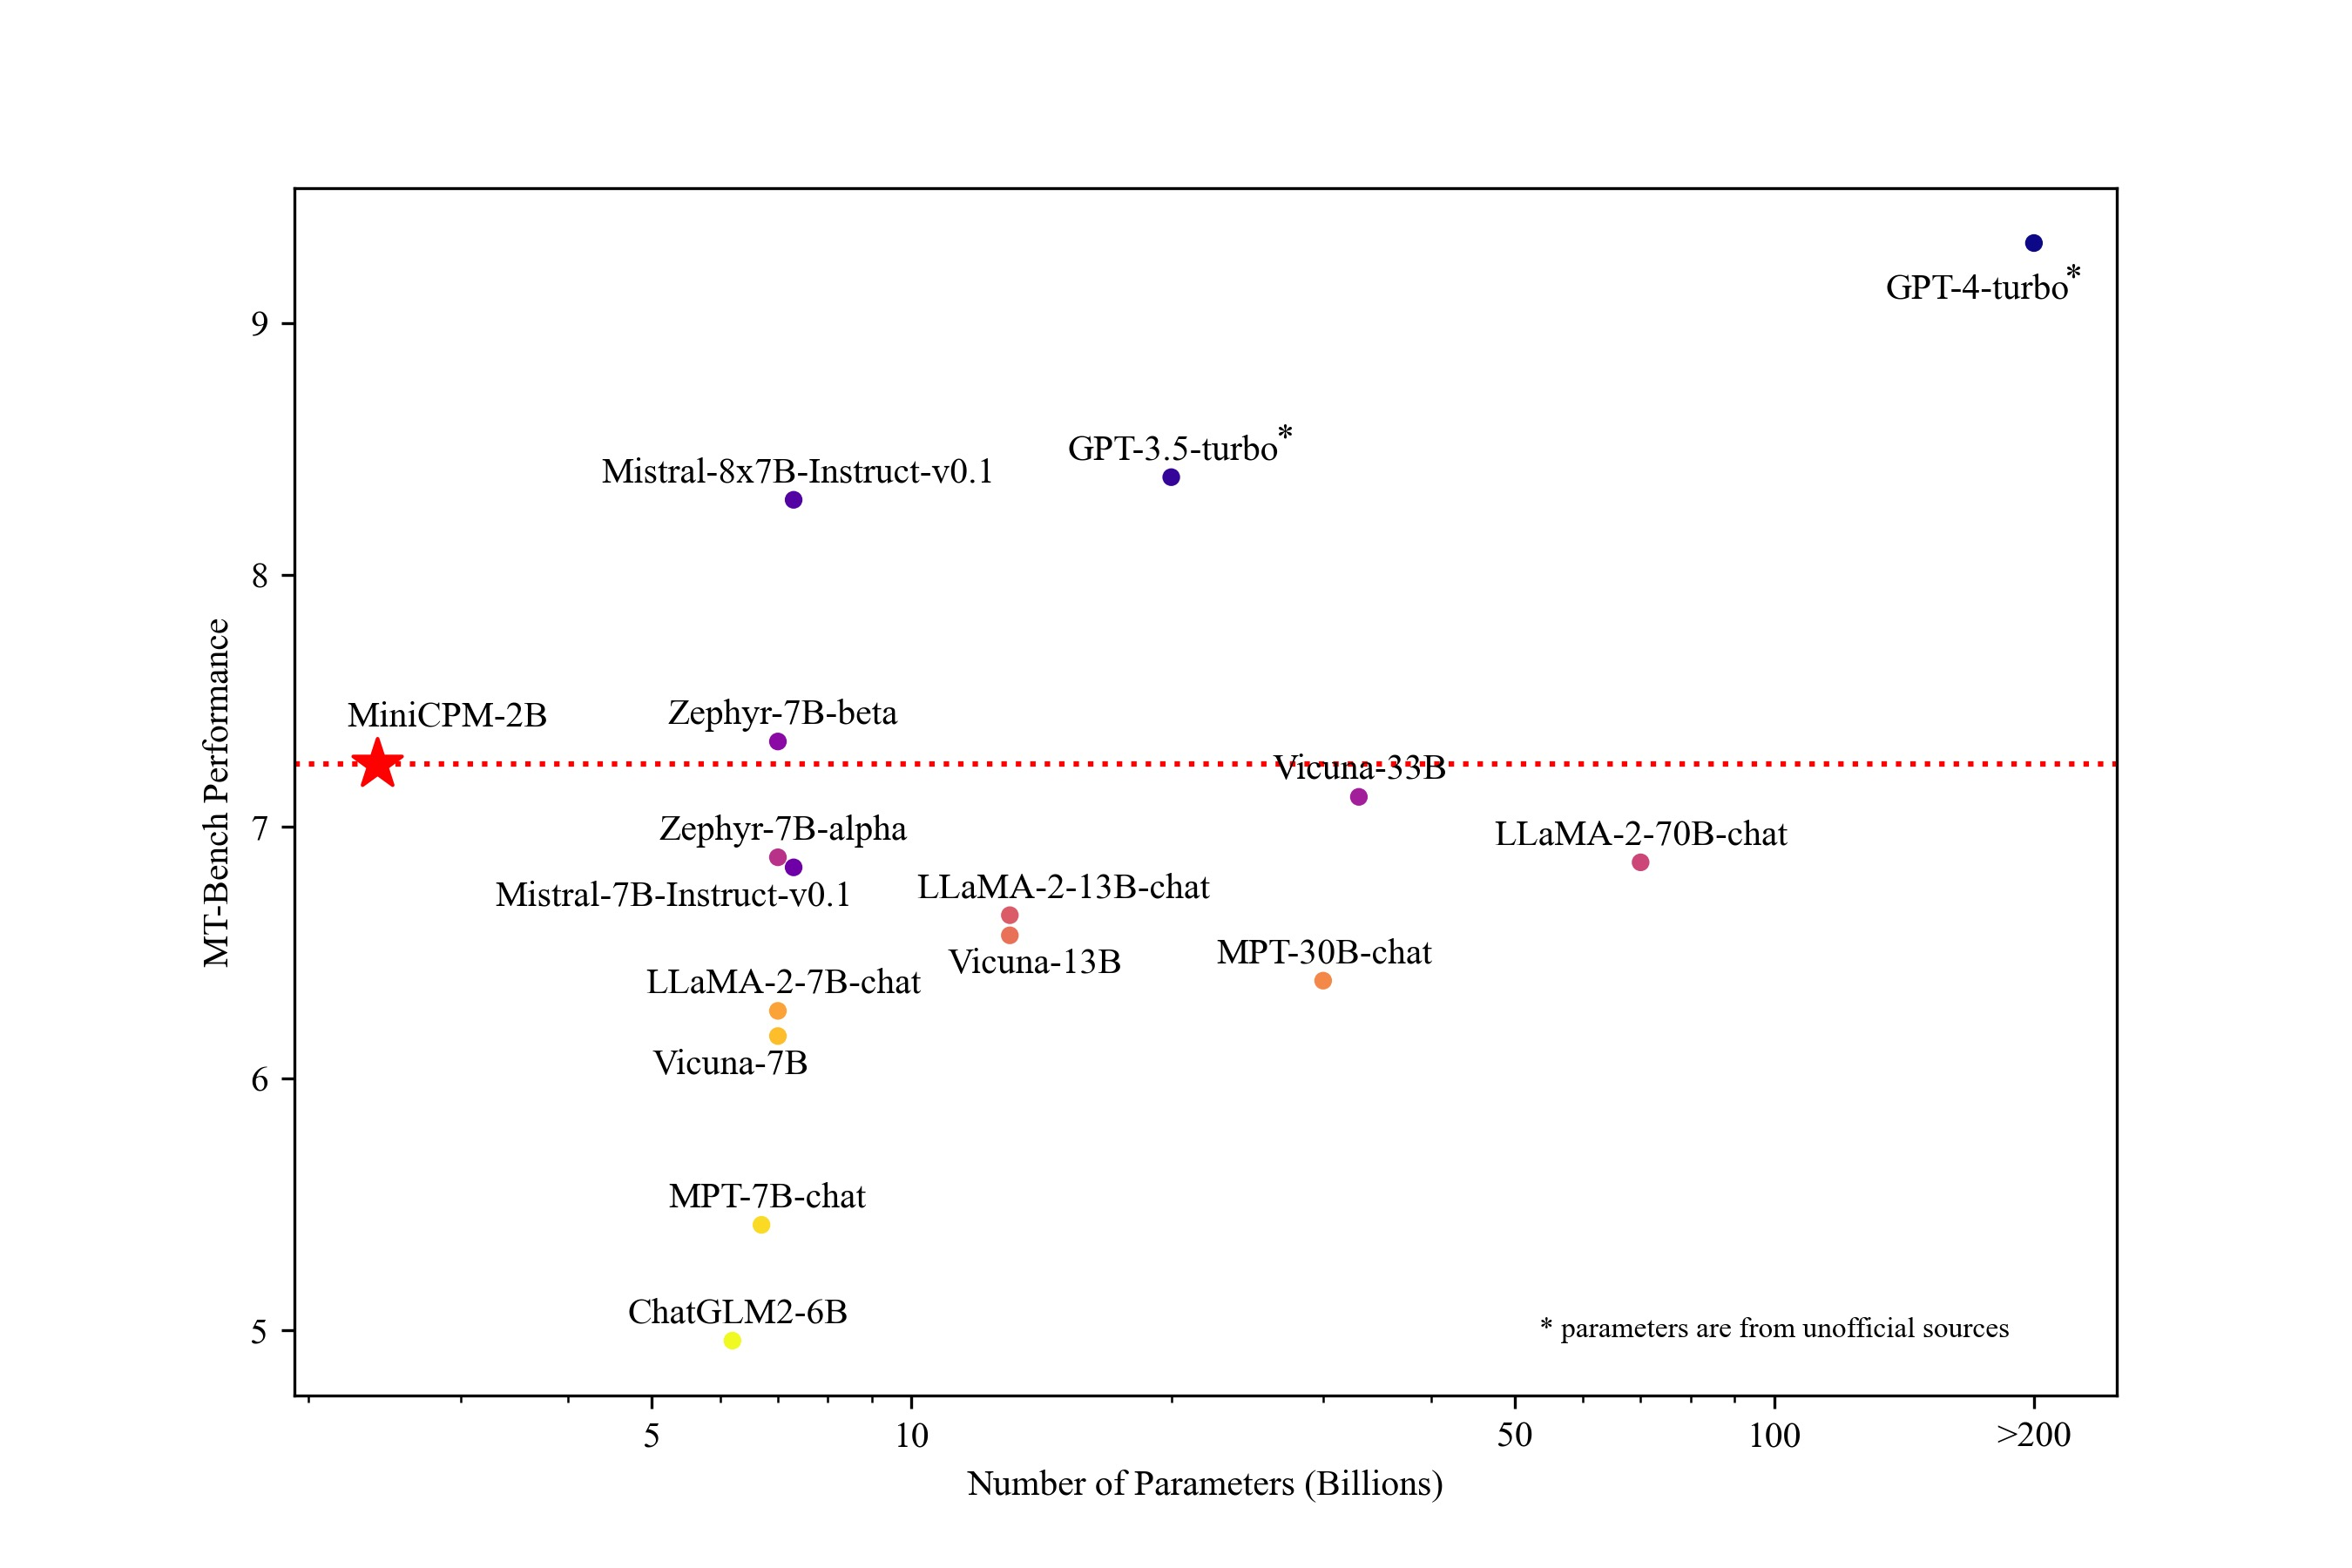
\includegraphics[width=0.7\linewidth]{Fig/mtbench_graph.jpg}
    \caption{MTBench score of MiniCPM-DPO-2.4B surpasses many models of larger size. }
    \label{fig:mtbenchscore}
    \vspace{-5mm}
\end{figure}
\subsection{MiniCPM-128K}

\textbf{Initialization.}
\uline{For the initialization, we disable sharing embeddings between input and output, primarily to accommodate vocabulary parallelism essential for training with long context.} \uline{The LM head is initialized from the input embedding.}

\textbf{Training.}
Similar to MiniCPM, MiniCPM-2.4B-128K utilizes the WSD as its learning rate scheduler and reuses the last checkpoint of the stable training stage of MiniCPM-2.4B. Concerning training data, we categorize the dataset distribution detailed in Section~\ref{sec:appdatadistrbution} into ``short data'' and ``long data''. \uline{We classify books, wikis, and papers as ``long data'', and the other as the ``short data''.} The training comprises 44\% long data and 56\% short data for continued training. \textbf{For the extension of long contexts, we apply Adjusted Base Frequency (ABF)~\citep{xiong2023effective} in the 4K to 32k range and employ NTK-Aware RoPE Scaling~\citep{bloc97_2023_ntk} and curriculum learning from 32K to 128K.} Both two stages involve future training. Furthermore, as indicated in Yi Tech Report~\citep{young2024yi} and Zebra~\citep{song2023zebra}, \uline{we use of synthetic long QA data that significantly enhances model performance in context-aware tasks.}

\textbf{Evaluation.} We evaluate MiniCPM-2.4B-128K in $\infty$Bench~\citep{zhang2024infty}, a pioneering benchmark for long context evaluations. \textbf{The tasks in $\infty$Bench~\citep{zhang2024infty} extend beyond typical retrieval tasks and challenge the model with long context reasoning.} We can see in Table~\ref{tab:longcontext}, we achieve comparable results in Mistral-7B-Instruct-v0.2 (ABF1000w) and outperform ChatGLM3-6B-128K despite being 2.5 times smaller.
\begin{table}[htpb]
\centering
\scalebox{0.82}{
\begin{tabular}
{m{4cm}m{1.2cm}m{1.2cm}m{1.2cm}m{1.2cm}m{1.2cm}m{1.2cm}m{1.2cm}}
\toprule
\textbf{Model}                               & \textbf{Passkey} & \textbf{Number String} & \textbf{KV Retrieval} & \textbf{Long Book Choice Eng} & \textbf{Long Book QA Chn} & \textbf{Long Book QA Eng }& \textbf{Long Book Sum Eng} \\
\midrule
LWM-Text-128K                       & 100     & 97.8           & 0.6           & 28.82                 & 15.93             & 14.31             & 9.99               \\
Yarn-Mistral-7b-128K                & 92.71   & 56.61          & 0             & 27.95                 & 15.49             & 9.55              & 9.06               \\
Mistral-7B-Instruct-v0.2(ABF 1000w) & 100     & 78.98          & 3.6           & 37.12                 & 11.74             & 17.37             & 21.12              \\
Yi-6B-200K                          & 100     & 94.92          & 0             & 36.68                 & 15.07             & 9.2               & 0.92               \\
ChatGLM3-6B-128K                    & 89.93   & 99.66          & 5.2           & 46.29                 & 10.7              & 8.38              & 25.91              \\
\midrule
\textbf{MiniCPM-2.4B-128K }                & 98.31   & 99.83          & 9             & 29.69                 & 23.06             & 16.33             & 15.73              \\
\bottomrule
\end{tabular}
}
\scalebox{0.83}{
\centering
\begin{tabular}{m{4cm}m{1.4cm}m{1.0cm}m{1.0cm}m{1.2cm}m{1.2cm}m{1.2cm}m{1.2cm}}
\toprule
\textbf{Model}                               & \textbf{Long Dialogue QA Eng} & \textbf{Math Calc} & \textbf{Math Find} & \textbf{Code Debug} & \textbf{Code Run} & \textbf{Avg} & \textbf{Avg w/o Code \& Math} \\
\midrule
LWM-Text-128k                       & 1.5                   & 0          & 3.43       & 20.05       & 1         & 24.45 & 33.62              \\
Yarn-Mistral-7b-128k                & 7.5                   & 0          & 17.14      & 0.76        & 1.25      & 19.84 & 27.36              \\
Mistral-7B-Instruct-v0.2(ABF 1000w) & 9.5                   & 0          & 29.43      & 17.51       & 0         & 27.75 & 36.9               \\
Yi-6B-200K                          & 3.5                   & 0          & 4.29       & 0.51        & 0.75      & 22.15 & 32.54              \\
ChatGLM3-6B-128K                    & 6.5                   & 0          & 8          & 5.33        & 1         & 25.58 & 36.57              \\
\midrule
\textbf{MiniCPM-2.4B-128K}                   & 9.5                   & 0          & 4.29       & 22.08       & 0         & 27.32 & 37.68              \\
\bottomrule
\end{tabular}
}
\caption{MiniCPM-2.4B-128K result in $\infty$Bench~\citep{zhang2024infty} }
\label{tab:longcontext}
\end{table}
\subsection{MiniCPM-MoE}

\textbf{Initialization.}
MiniCPM-MoE is initialized utilizing Sparse Upcycling~\citep{komatsuzaki2022sparse}. \uline{The dense model checkpoint, derived from the stable phase of MiniCPM, undergoes a transformation wherein each MLP layer is substituted by an MoE layer.} \uline{These new MoE layers are exact replicas of the original MLP layers from the dense checkpoint.} \uline{The router parameters are randomly initialized following a normal distribution with a mean of 0 and a variance of 0.01.}

\textbf{Routing Mechanism.}
The number of total non-embedding parameters of MiniCPM-MoE is 13.6B. 
During training and inference, two out of eight experts are activated for each token, resulting in the number of activated parameters being approximately 4B. To prevent training from collapsing, an additional load balancing loss~\citep{fedus2022switch} is applied to the final training objective. This auxiliary loss is multiplied by 0.01 which is large enough to ensure a balanced distribution of tokens assigned to different experts.

\textbf{Training.}
 Similar to MiniCPM, we employ WSD as our learning rate scheduler. Regarding the training data, we adhere strictly to the distribution specified in Section \ref{sec:appdatadistrbution}. The training batch size is maintained at 4M tokens during the stable training and decay stages and is reduced to 2M tokens during the SFT stage. The pre-training phase (including continue pre-train and decay stage) spans 130K steps, after which we notice diminishing improvement. The benchmark results are detailed in Table \ref{tab:a4_moe_benchmark}.


\begin{table}[htbp]
    \centering
\scalebox{0.80}{
    \begin{tabular}{l|cccccccc}
\toprule
    \textbf{Model} &  \textbf{C-Eval} & \textbf{CMMLU} & \textbf{MMLU} & \textbf{HumanEval} & \textbf{MBPP} & \textbf{GSM8K} & \textbf{MATH} &\textbf{BBH}  \\
\midrule
    Llama2-34B & - & - & 62.6 & 22.6 & 33.0$^\dag$ & 42.2 & 6.24 & \textbf{44.1} \\
    Deepseek-MoE (16B) & 40.6 & 42.5 & 45.0 & 26.8 & 39.2 & 18.8 & 4.3 &  - \\
    Mistral-7B & 46.12 & 42.96 & \textbf{62.69} & 27.44 & 45.20 & 33.13 & 5.0 & {41.06 }\\
    Gemma-7B & 42.57 & 44.20 & 60.83 & 38.41 & 50.12 & 47.31 & 6.18 & 39.19 \\
\midrule
    MiniCPM-2.4B & 51.13 & 51.07 & 53.46 & 50.00 & 47.31 & 53.83 & 10.24 & 36.87 \\
   \textbf{MiniCPM-MoE (13.6B)} & \textbf{58.11} & \textbf{58.80} & 58.90 & \textbf{56.71} & \textbf{51.05} & \textbf{61.56} & \textbf{10.52} & 39.22 \\
\bottomrule

    \end{tabular}
}
    \caption{Benchmark results of MiniCPM-MoE. $^\dag$ means evaluation results on the full set of MBPP, instead of the hand-verified set~\citep{austin2021program}. The evaluation results of Llama2-34B and Qwen1.5-7B are taken from their technical reports.}
    \label{tab:a4_moe_benchmark}

\end{table}


